 %%%%%%%%%%%%%%%%%%%%%%%%%%%%%%%%%%%%%%%%%%%%%%%%%%%%%%%%%%%%%%%%%%%%%%
% LaTeX Example: Project Report
%
% Source: http://www.howtotex.com
%
% Feel free to distribute this example, but please keep the referral
% to howtotex.com
% Date: March 2011 
% 
%%%%%%%%%%%%%%%%%%%%%%%%%%%%%%%%%%%%%%%%%%%%%%%%%%%%%%%%%%%%%%%%%%%%%%
% How to use writeLaTeX: 
%
% You edit the source code here on the left, and the preview on the
% right shows you the result within a few seconds.
%
% Bookmark this page and share the URL with your co-authors. They can
% edit at the same time!
%
% You can upload figures, bibliographies, custom classes and
% styles using the files menu.
%
% If you're new to LaTeX, the wikibook is a great place to start:
% http://en.wikibooks.org/wiki/LaTeX
%
%%%%%%%%%%%%%%%%%%%%%%%%%%%%%%%%%%%%%%%%%%%%%%%%%%%%%%%%%%%%%%%%%%%%%%
% Edit the title below to update the display in My Documents
%\title{Project Report}
%
%%% Preamble
\documentclass[paper=a4, fontsize=11pt]{scrartcl}
\usepackage[T1]{fontenc}
\usepackage{fourier}
\usepackage{tabularx}
\usepackage[utf8]{inputenc}
\usepackage{hyperref}

\usepackage{graphicx}
\usepackage{caption}
\usepackage{subcaption}

\usepackage[english]{babel}															% English language/hyphenation
\usepackage[protrusion=true,expansion=true]{microtype}	
\usepackage{amsmath,amsfonts,amsthm} % Math packages

\usepackage{url}
%\usepackage[hang, small,labelfont=bf,up,textfont=it,up]{caption}


%%% Custom sectioning
\usepackage{sectsty}
\allsectionsfont{\normalfont\scshape}
\usepackage{float}
\usepackage{amsmath}
\usepackage{mathtools}



%%% Custom headers/footers (fancyhdr package)
\usepackage{fancyhdr}
\pagestyle{fancyplain}
\fancyhead{}											% No page header
\fancyfoot[L]{}											% Empty 
\fancyfoot[C]{}											% Empty
\fancyfoot[R]{\thepage}									% Pagenumbering
\renewcommand{\headrulewidth}{0pt}			% Remove header underlines
\renewcommand{\footrulewidth}{0pt}				% Remove footer underlines
\setlength{\headheight}{13.6pt}


%%% Equation and float numbering
\numberwithin{equation}{section}		% Equationnumbering: section.eq#
\numberwithin{figure}{section}			% Figurenumbering: section.fig#
\numberwithin{table}{section}				% Tablenumbering: section.tab#


%%% Maketitle metadata

\newcommand{\horrule}[1]{\rule{\linewidth}{#1}} 	% Horizontal rule

\title{
		%\vspace{-1in} 	
		\usefont{OT1}{bch}{b}{n}
		\normalfont \normalsize \textsc{} \\ [25pt]
		
\includegraphics[width=0.4\linewidth]{tru}		
		\horrule{0.5pt} \\[0.2cm]
		\huge Nucleon Decay Generator Validation \\
		\horrule{2pt} \\[0.005cm]
}
\author{
		\normalfont 								\normalsize
        Jerin Roberts\\[-5pt]		\normalsize
        \today
}
\date{}




%%% Begin document
\begin{document}
\maketitle
\begin{center}
\begin{tabular}{l r}


Supervisors: & Dr. Christine Kraus, Dr. Erica Caden  \\ % supervisor
Locations: & SNOLAB, Laurentian University


\end{tabular}
\end{center}
\newpage
\tableofcontents
\listoffigures
\listoftables
\newpage
\section{Introduction}
The SNO+ experiment will be used to search for rare modes of radioactive decay. These modes which typically violate baryon and lepton number conservations, if discovered could help explain the antimatter and matter asymmetries seen through out the universe. 
\section{Neutrino-less double Beta Decay}The experiment is broken into two phases; water and scintillation phase. During scintillation phase SNO+ will search for the rare neutrino-less double beta decay. Linear Alkyl Benzene will be loaded at 0.5\% with a tellurium isotope. During regular beta decay a electron and a neutrino are given off both which which take a portion of the released energy. This generates a spectrum of energies for the detected electrons. During a neutrino-less double beta decay the neutrinos interected and anilate each other leaving just a double electron emission. Since the neutrinos are never ejected the energy released is given complettly to the electrons which results in the descrete energy spectrum. SNO+ will search for this small yet detectable blip in the electron energy emission spectrum.
\section{Invisible Nucleon Decay} 

During the water phase SNO+ will search for rare invisible nucleon decay. 

\begin{figure}[h]
        \centering
        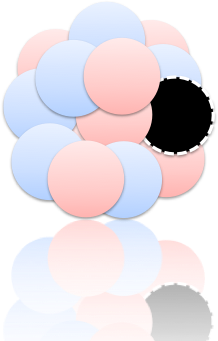
\includegraphics[height=3cm]{nuc}
        \caption{Displays an exited atom after a nucleon decay}
        \label{nuc}
\end{figure} 




\begin{thebibliography}{99} % Beamer does not support BibTeX so references must be inserted manually as below
\bibitem[Garcia, 2014]{picfsk} Lawrence Garcia (2014)
\newblock Umbilical Tests and Detector Data Analysis


\bibitem[Maneira, 2013]{p1} Jose Maneira, Rui Alves (2013)
\newblock URM design for SNO+, LIP-Coimbra

\end{thebibliography}


%%% End document
\end{document}